% The appendix or appendices should contain your group meeting minutes and any additional raw material that is referred to in the text (e.g. data from requirements gathering, paper prototypes etc.)

\section{Prototyping}
\subsection{AR Prototypes}
\subsubsection{Vuforia}
\begin{figure}[H]
\centering  
\begin{tabular}{cc}
  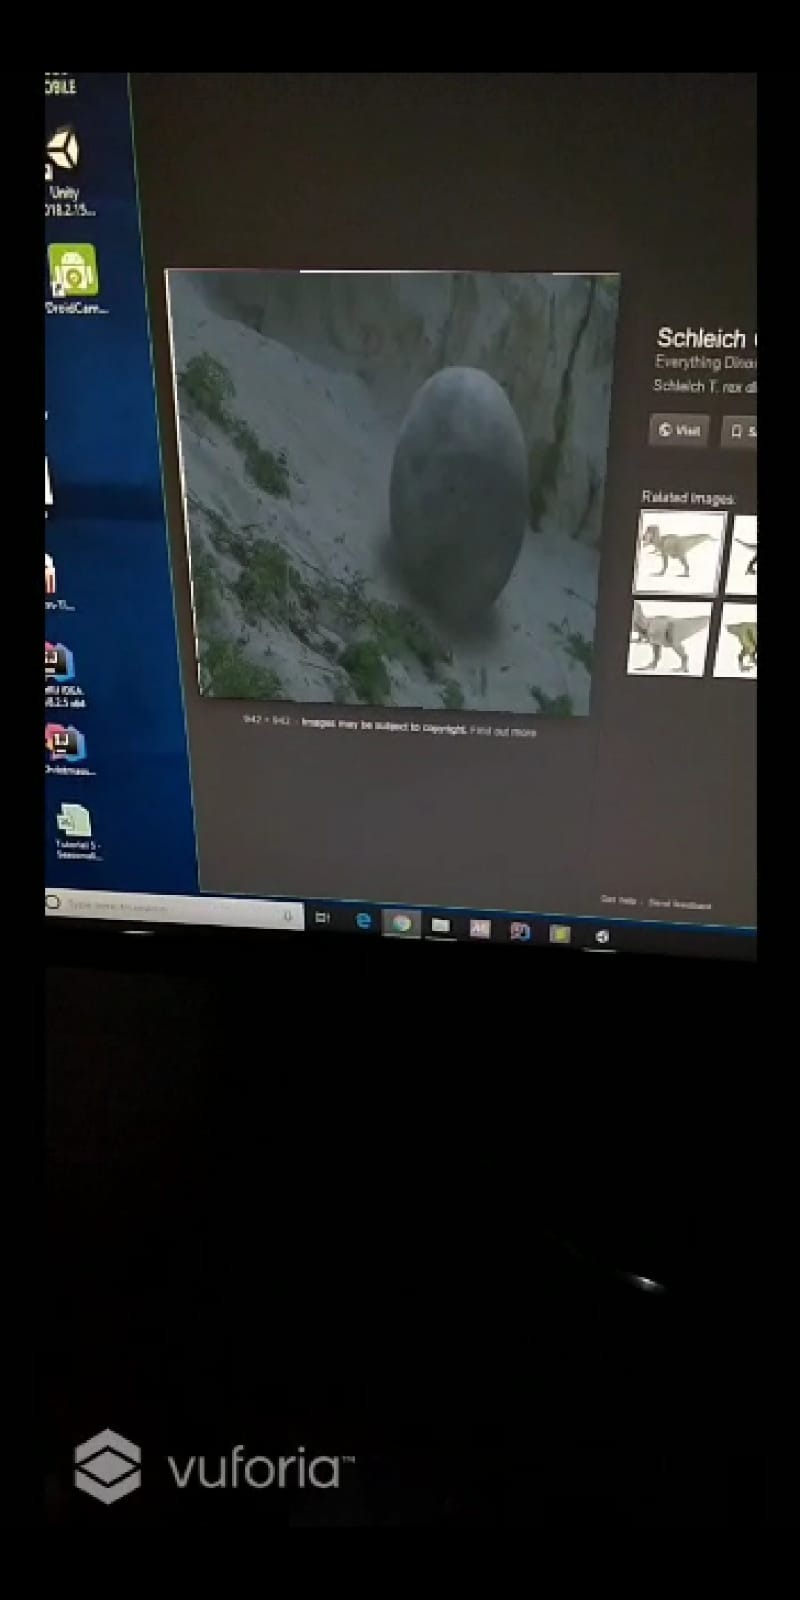
\includegraphics[width=60mm, height=100mm]{prototypes/ar/vulforia/1.jpeg} &   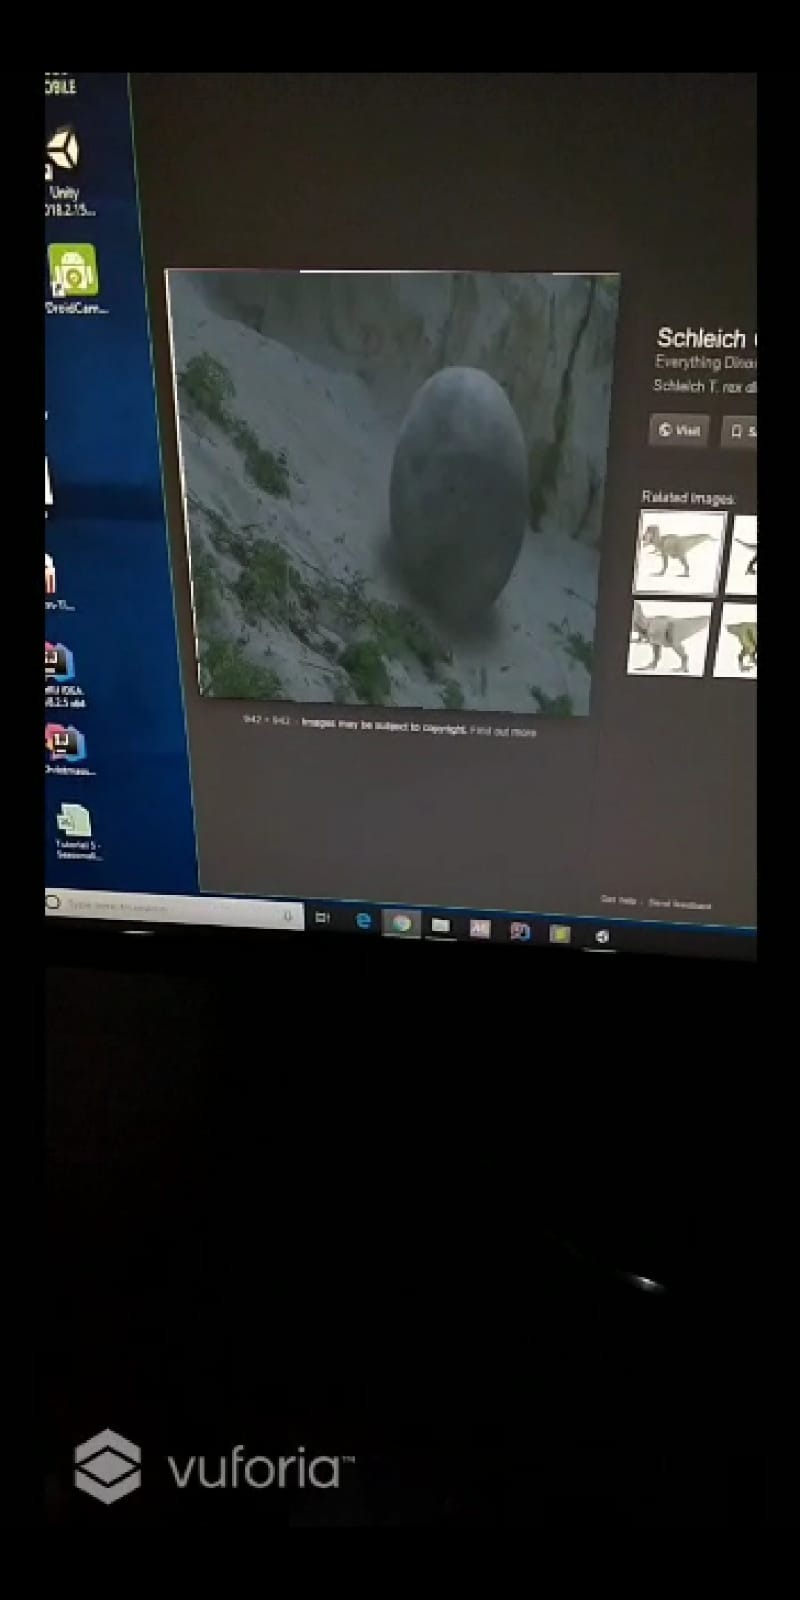
\includegraphics[width=60mm, height=100mm]{prototypes/ar/vulforia/2.jpeg} \\
(a) Camera over image & (b) Video superimposed on top of image\\[6pt]
\end{tabular}
\caption{Vuforia prototyping on Android device}
\label{fig:vulforia}
\end{figure}

\newpage
\subsubsection{ARKit}
\begin{figure}[H]
\centering  
\begin{tabular}{cc}
  \includegraphics[width=60mm, height=100mm]{prototypes/ar/ios/1.png} &   \includegraphics[width=60mm, height=100mm]{prototypes/ar/ios/2.png} \\
(a) Camera over image & (b) Image recognised and displaying information \\[6pt]
\multicolumn{2}{c}{\includegraphics[width=60mm, height=100mm]{prototypes/ar/ios/3.png} }\\
\multicolumn{2}{c}{(c) Image scanned before; showing the green tick}
\end{tabular}
\caption{ARKit prototyping on iOS device}
\label{fig:ARKit}
\end{figure}

\newpage
\subsubsection{ARCore}
\begin{figure}[H]
\centering  
\begin{tabular}{cc}
  
\includegraphics[width=60mm, height=100mm]{prototypes/ar/android/1.jpg} &   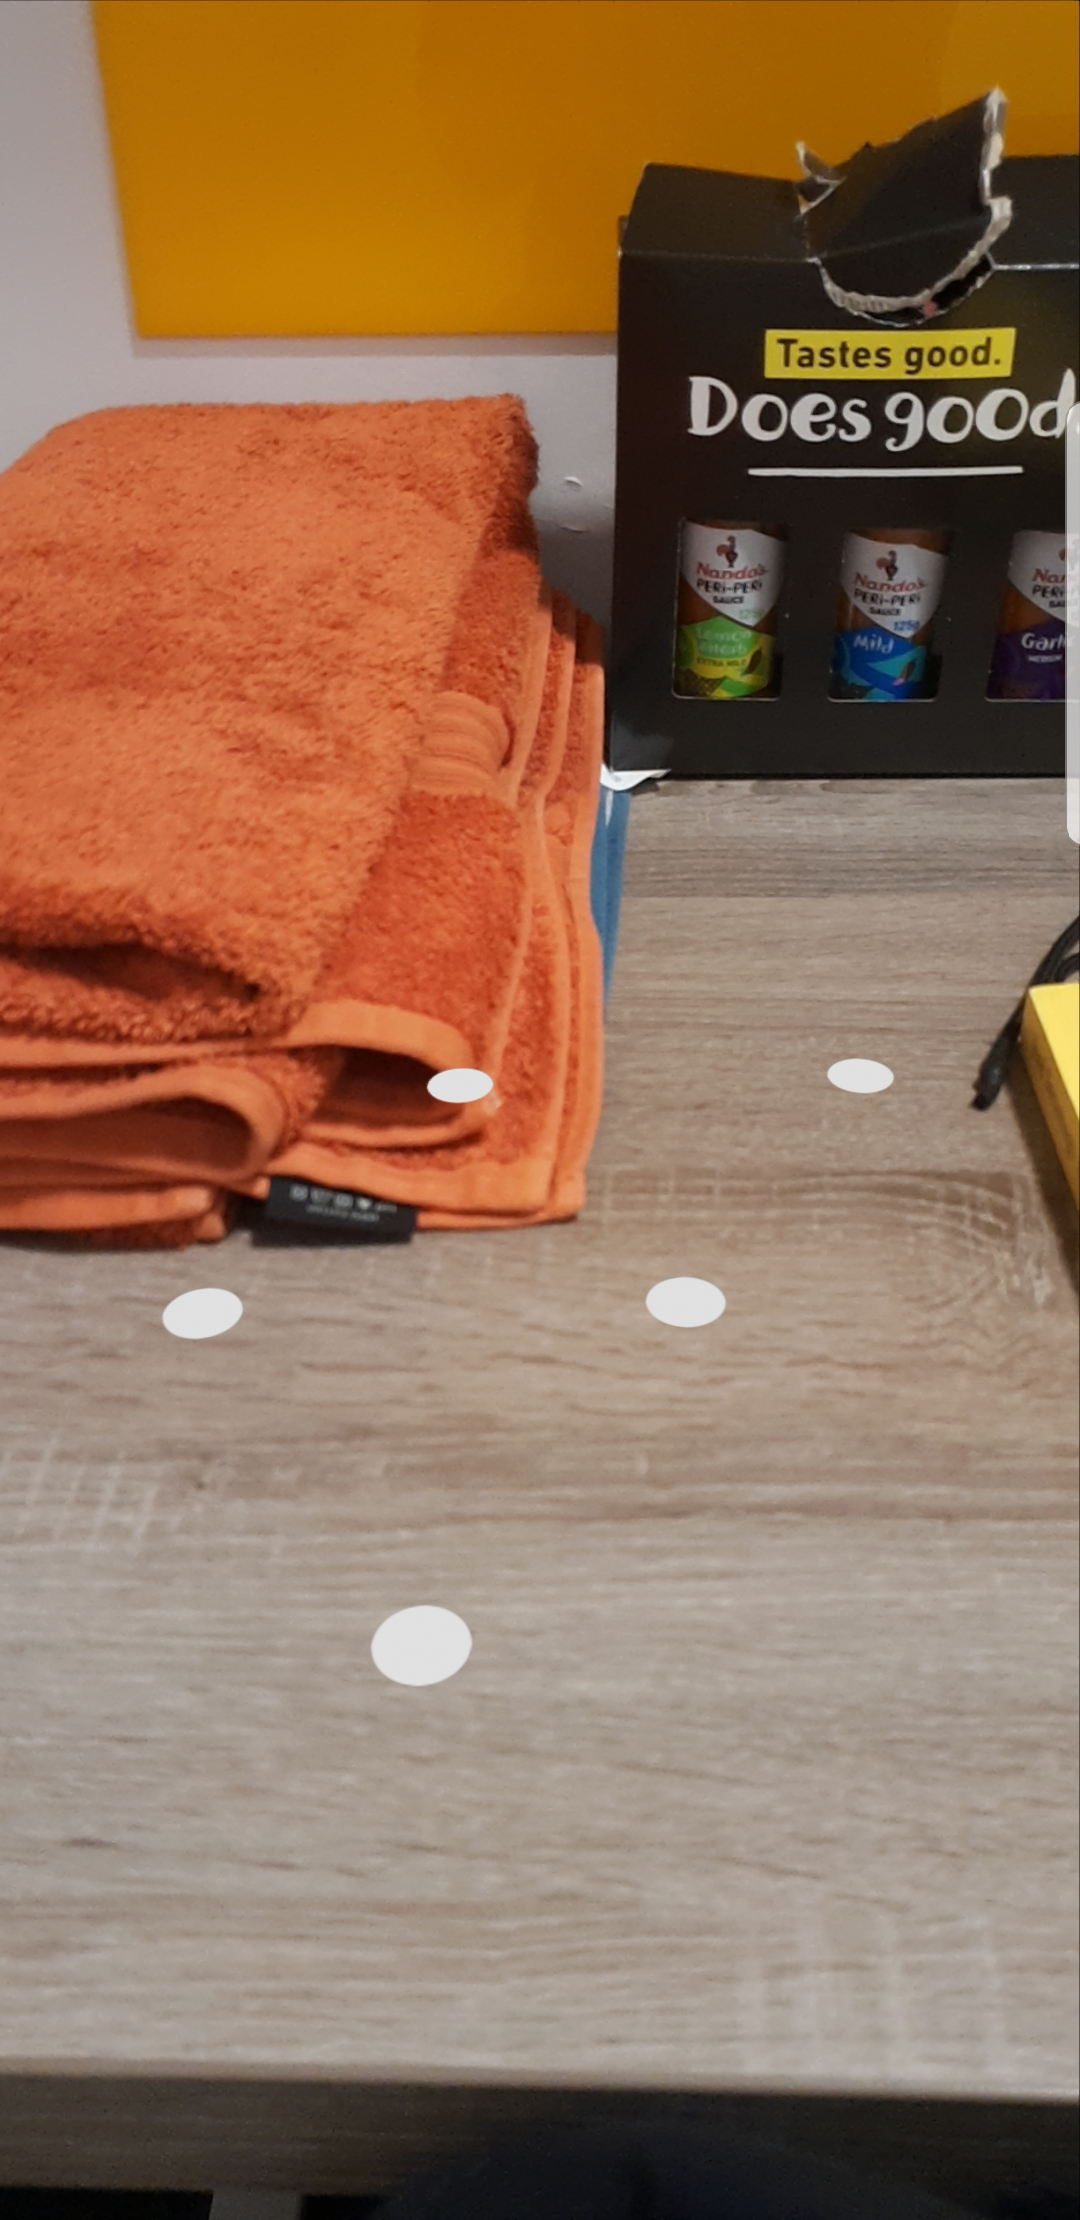
\includegraphics[width=60mm, height=100mm]{prototypes/ar/android/2.jpg} \\
(a) Initial view & (b) Detection of surface \\[6pt]
\multicolumn{2}{c}{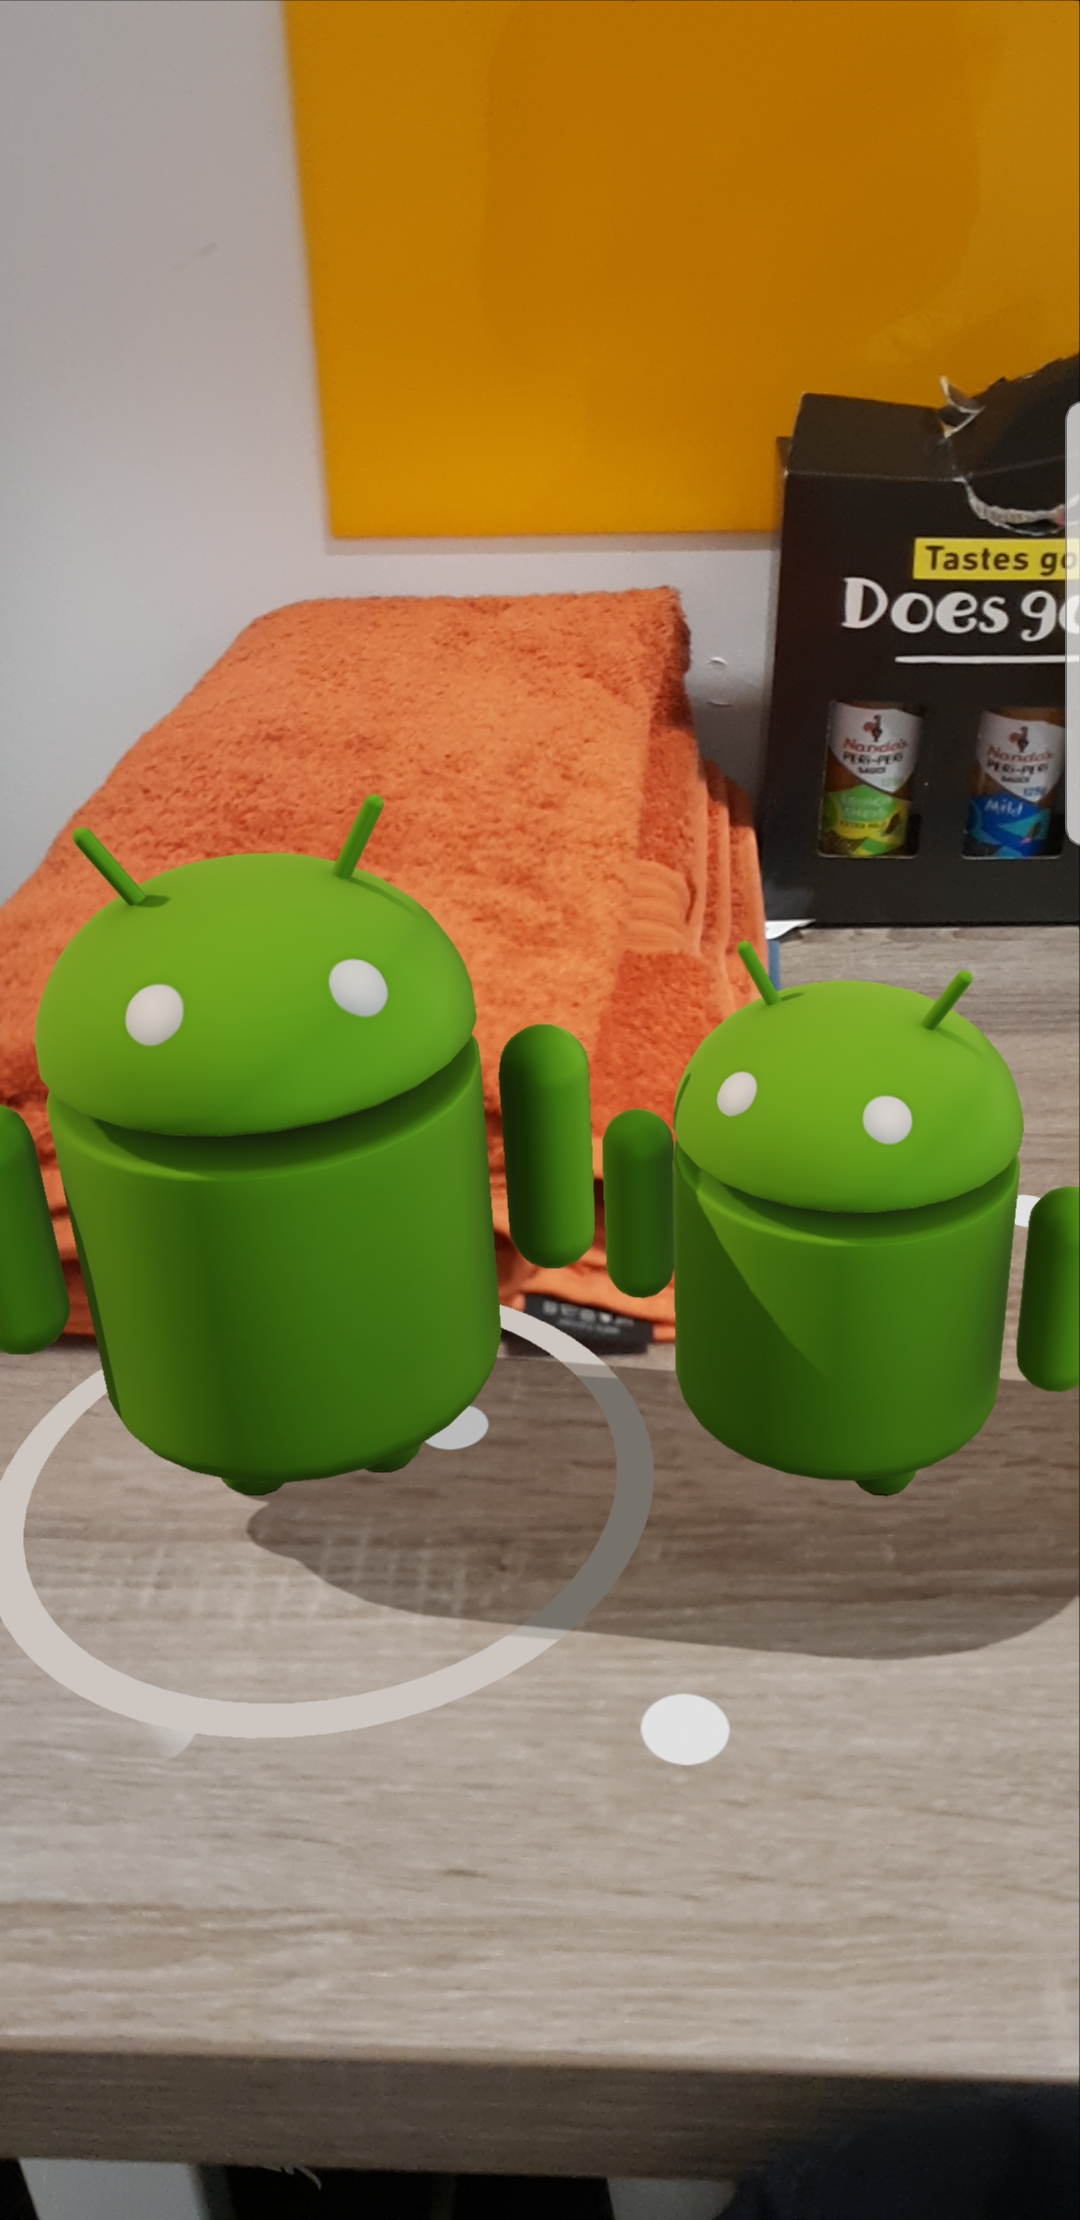
\includegraphics[width=60mm, height=100mm]{prototypes/ar/android/3.jpg} }\\
\multicolumn{2}{c}{(c) Objects superimposed on surface}
\end{tabular}
\caption{ARCore prototyping on Android device}
\label{fig:ARCore}
\end{figure}

\newpage
\subsubsection{Android Sensors Logging}
\begin{figure}[H]
    \centering
    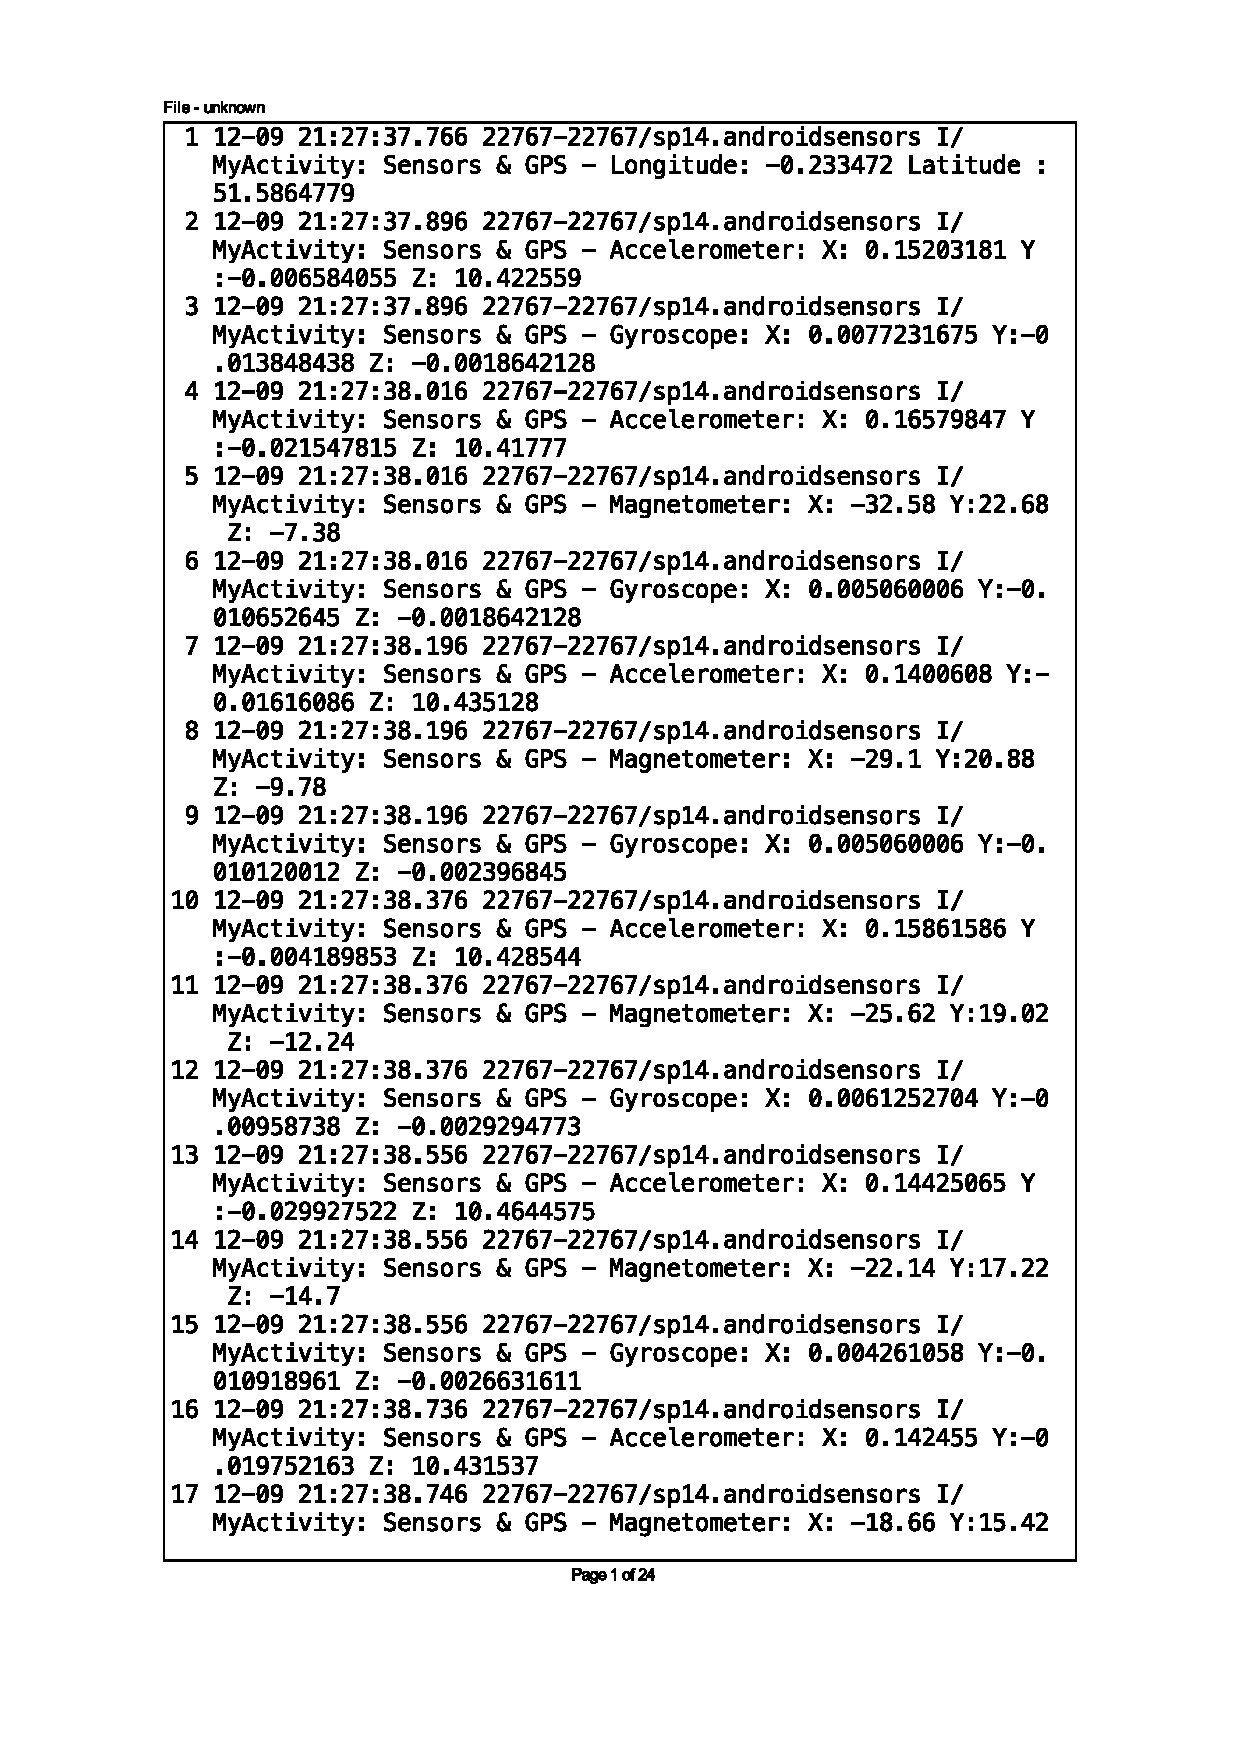
\includegraphics[width=\textwidth]
    {prototypes/ar/android/logs.pdf}
    \caption{GPS, accelerometer, magnometer, and gyroscope sensor data from an Android device over 1 second period}
    \label{fig:Android sensors logging}
\end{figure}

\subsection{UI/UX Prototypes}
\subsubsection{Storyboard}
\begin{figure}[H]
    \centering
    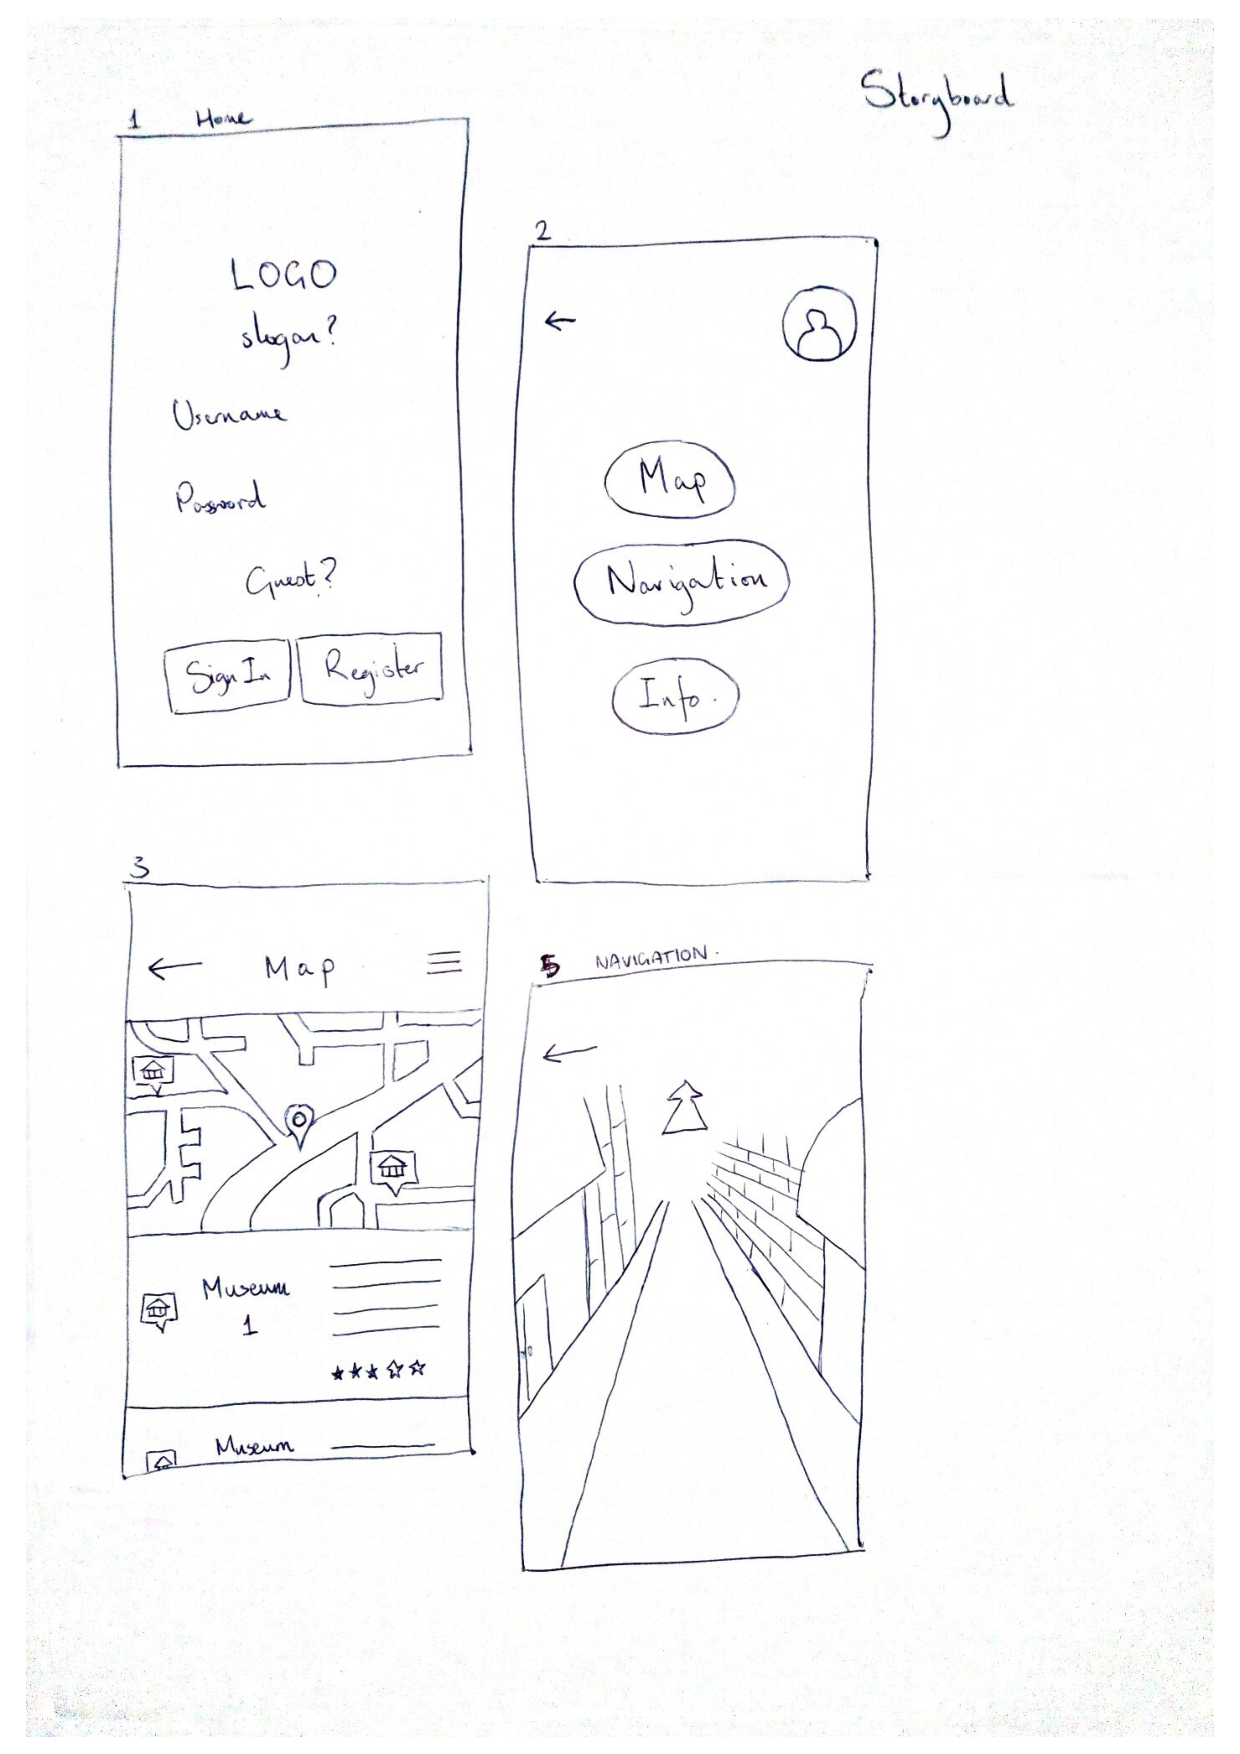
\includegraphics[width=\textwidth]
    {prototypes/ui/storyboard/1.pdf}
    \caption{Storyboard UI Drawings}
    \label{fig:storyboard}
\end{figure}

\newpage
\begin{figure}[H]
    \centering
    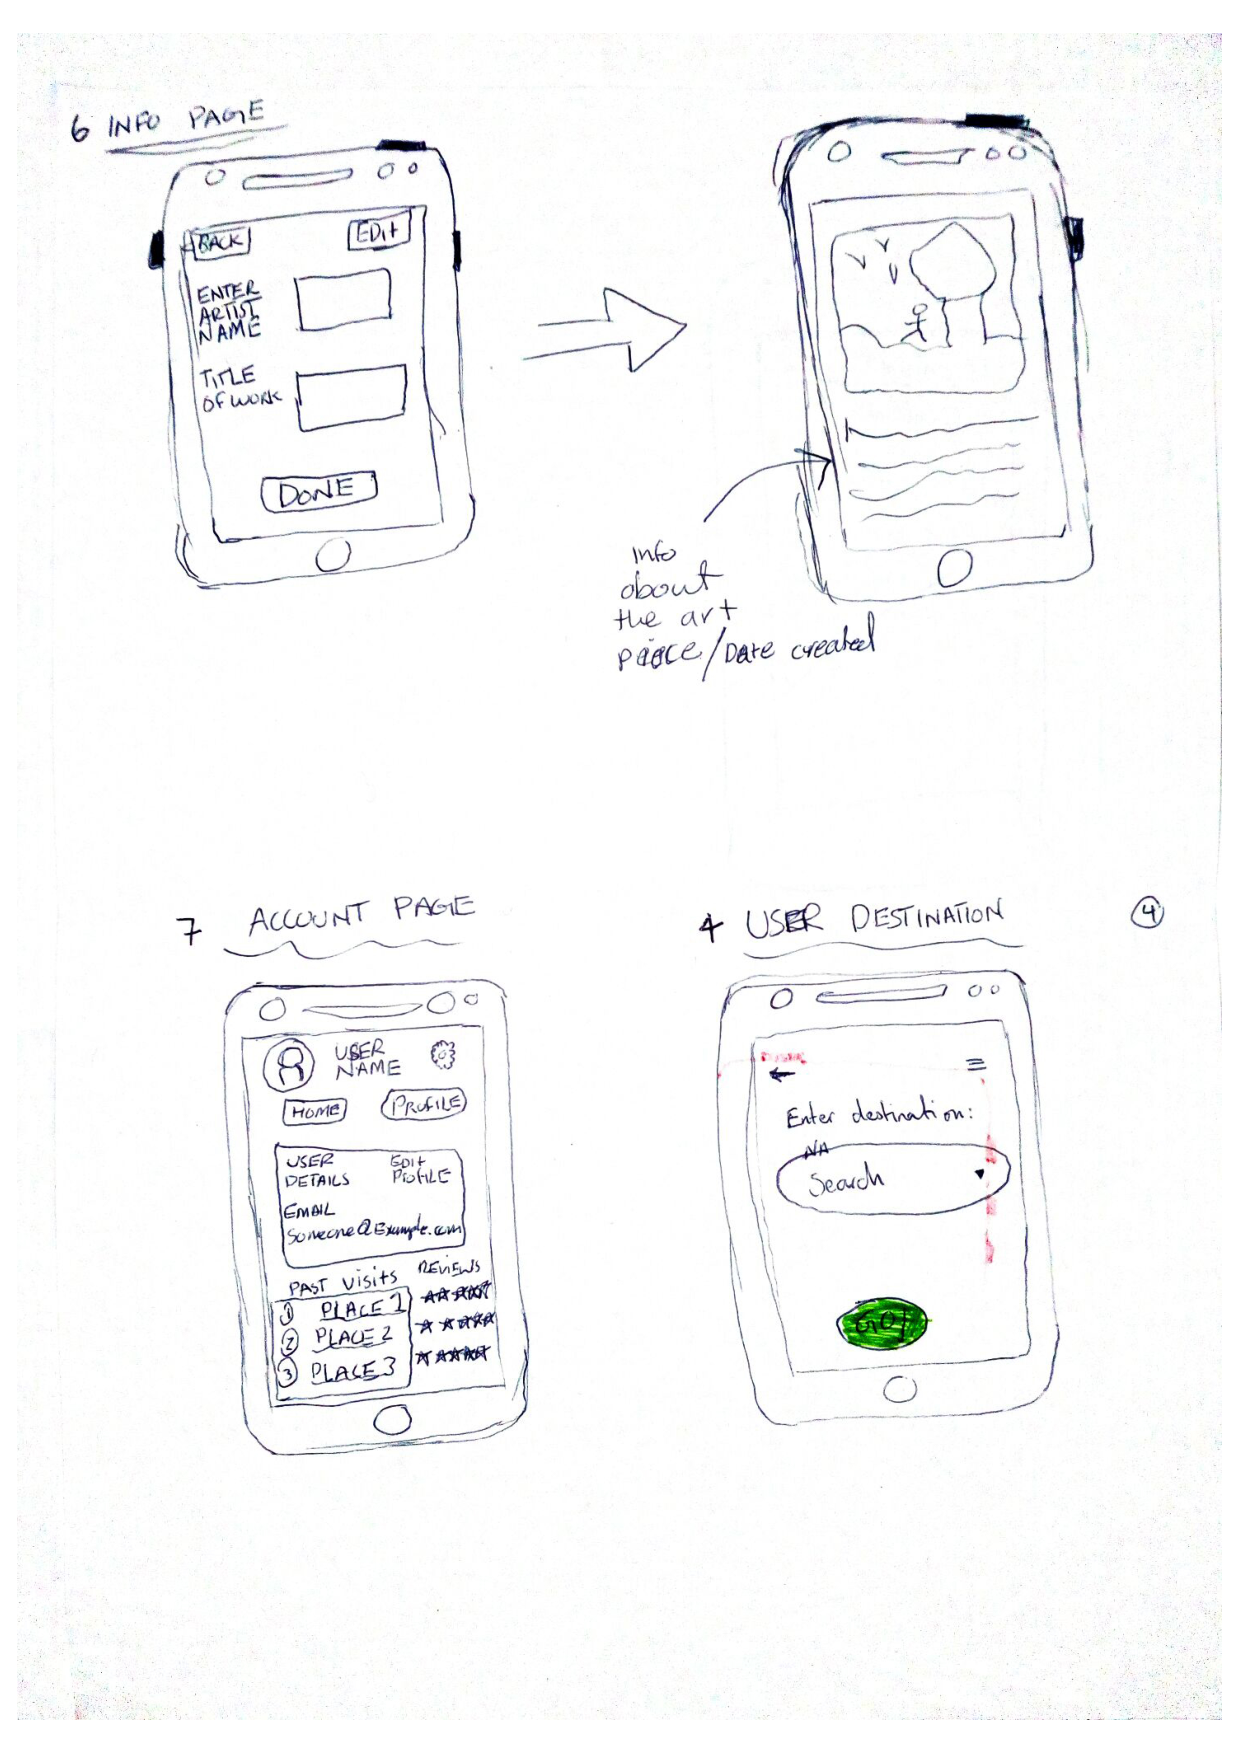
\includegraphics[width=\textwidth]
    {prototypes/ui/storyboard/2.pdf}
\end{figure}

\newpage
\begin{figure}[H]
    \centering
    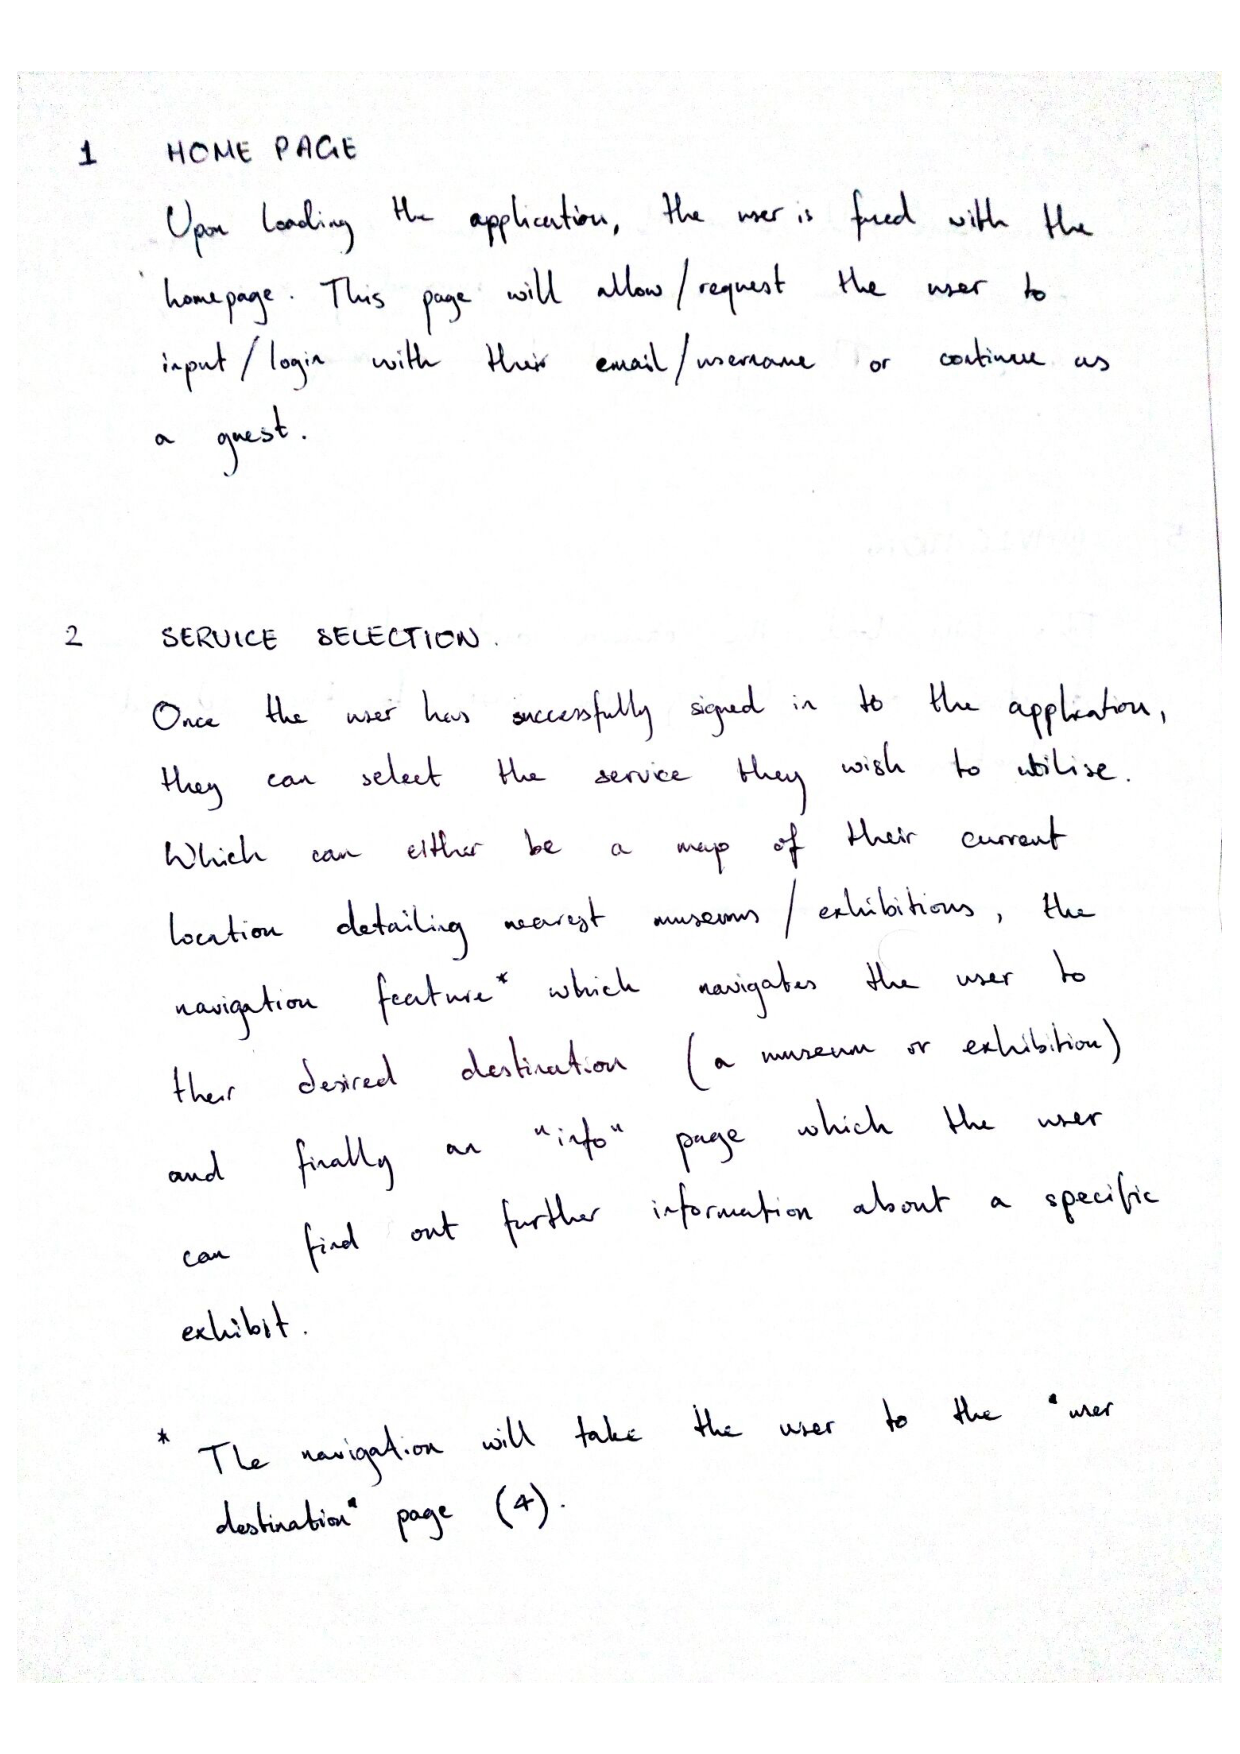
\includegraphics[width=\textwidth]
    {prototypes/ui/storyboard/3.pdf}
    \caption{Storyboard UI Descriptions}
\end{figure}

\newpage
\begin{figure}[H]
    \centering
    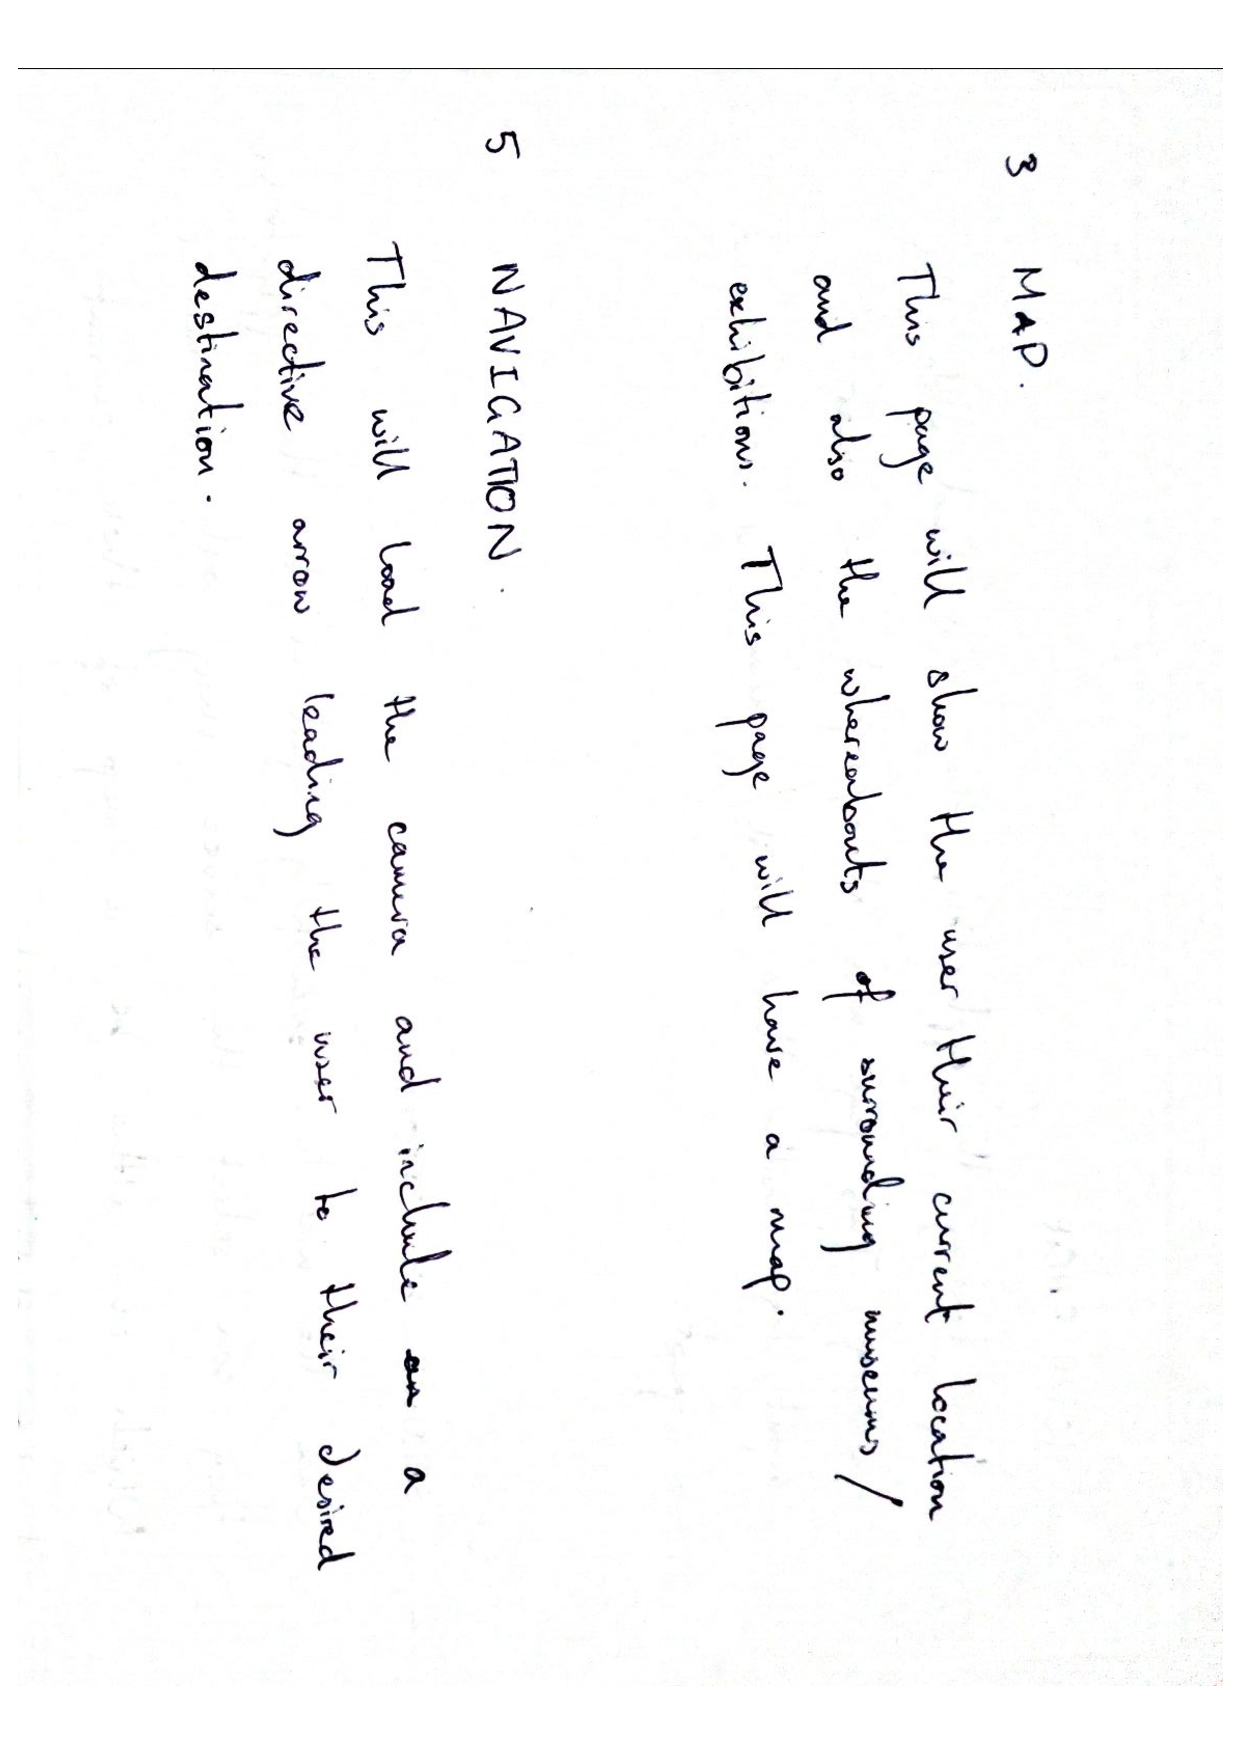
\includegraphics[angle=90, width=\textwidth]
    {prototypes/ui/storyboard/4.pdf}
\end{figure}

\newpage
\begin{figure}[H]
    \centering
    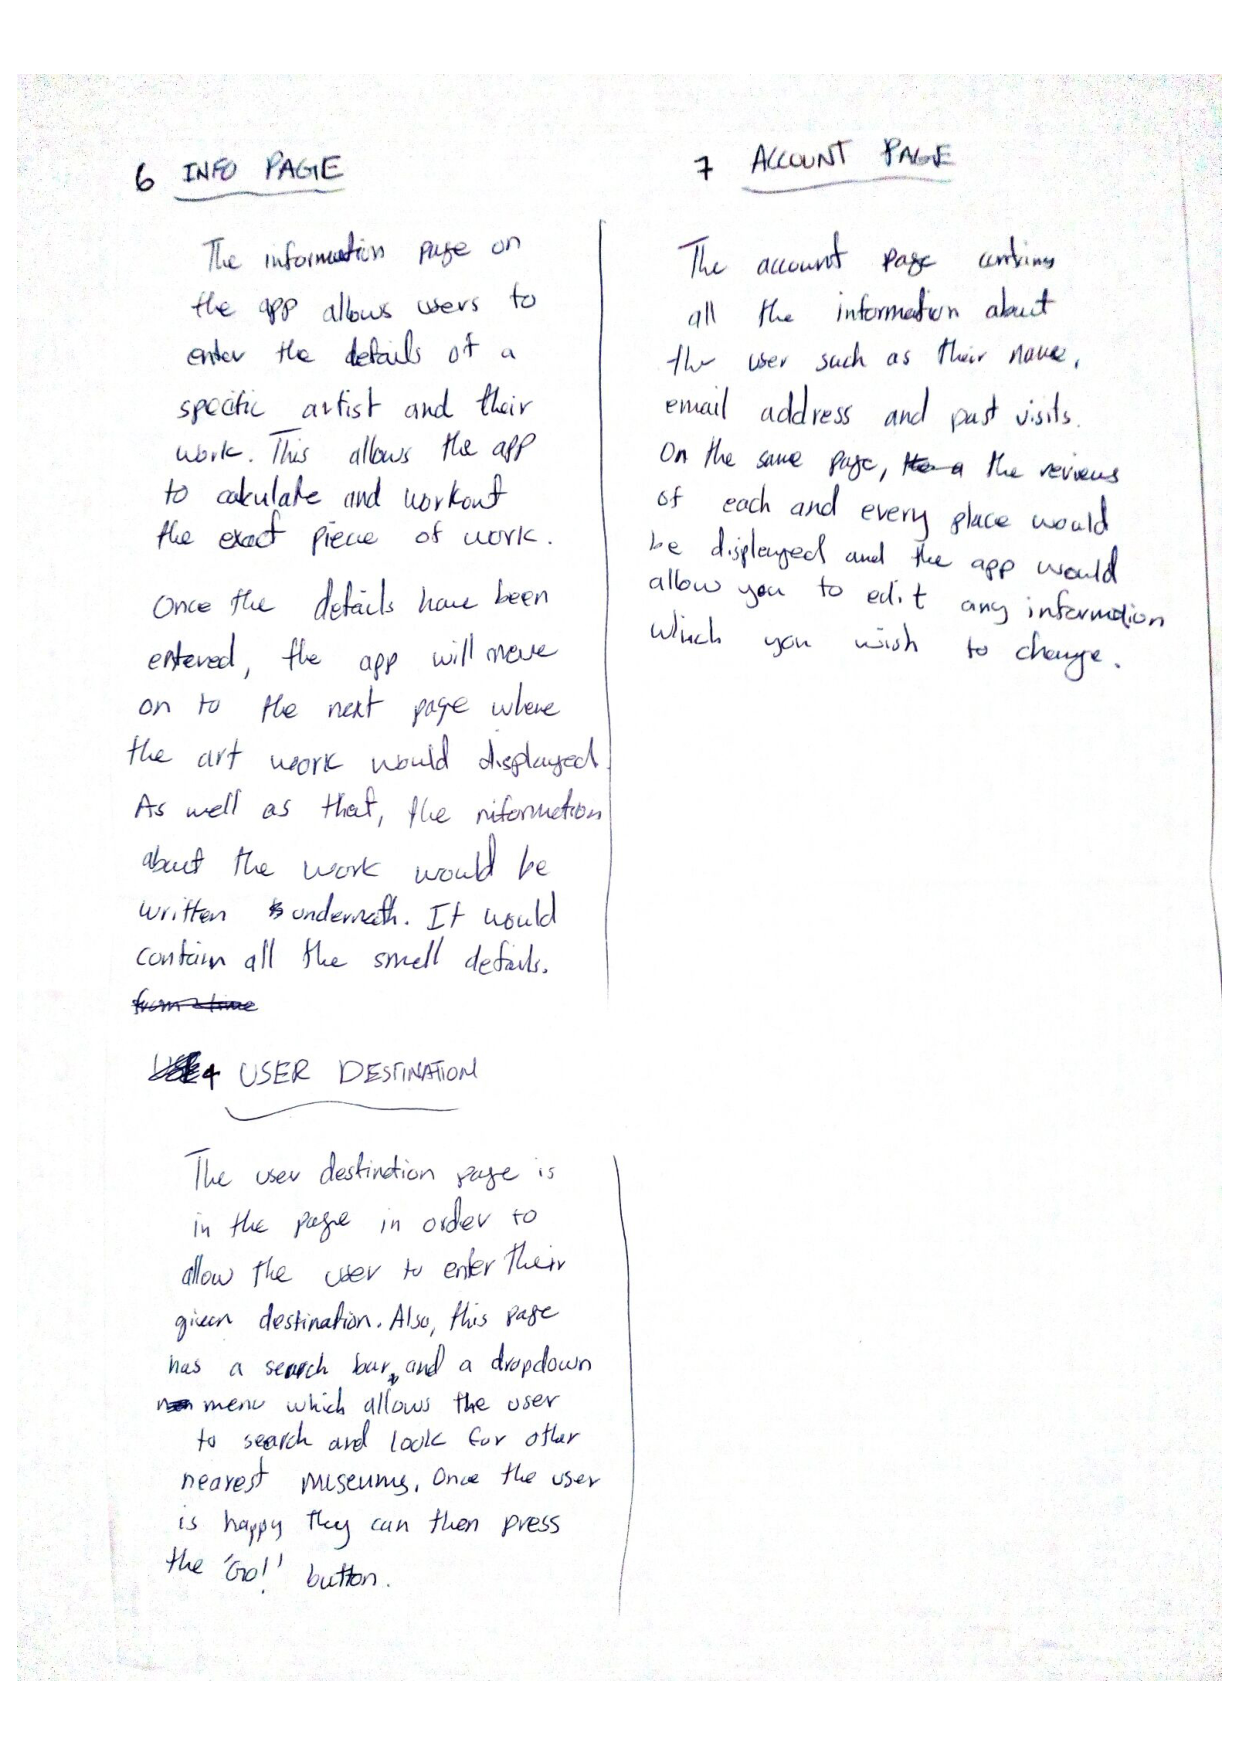
\includegraphics[width=\textwidth]
    {prototypes/ui/storyboard/5.pdf}
\end{figure}

\subsubsection{Prototype 1}
\begin{figure}[H]
    \centering
    \includegraphics[width=\textwidth]
    {prototypes/ui/1.png}
    \caption{Overview of UI Prototype 1}
    \label{fig:prototype1}
\end{figure}

\subsubsection{Prototype 2}
\begin{figure}[H]
    \centering
    \includegraphics[width=\textwidth]
    {prototypes/ui/2.png}
    \caption{Overview of UI Prototype 2}
    \label{fig:prototype2}
\end{figure}

\subsubsection{Prototype 3}
\begin{figure}[H]
    \centering
    \includegraphics[width=\textwidth]
    {prototypes/ui/3.png}
    \caption{Overview of UI Prototype 3}
    \label{fig:prototype3}
\end{figure}

\newpage
\subsubsection{Final Prototype}
\begin{figure}[H]
    \centering
    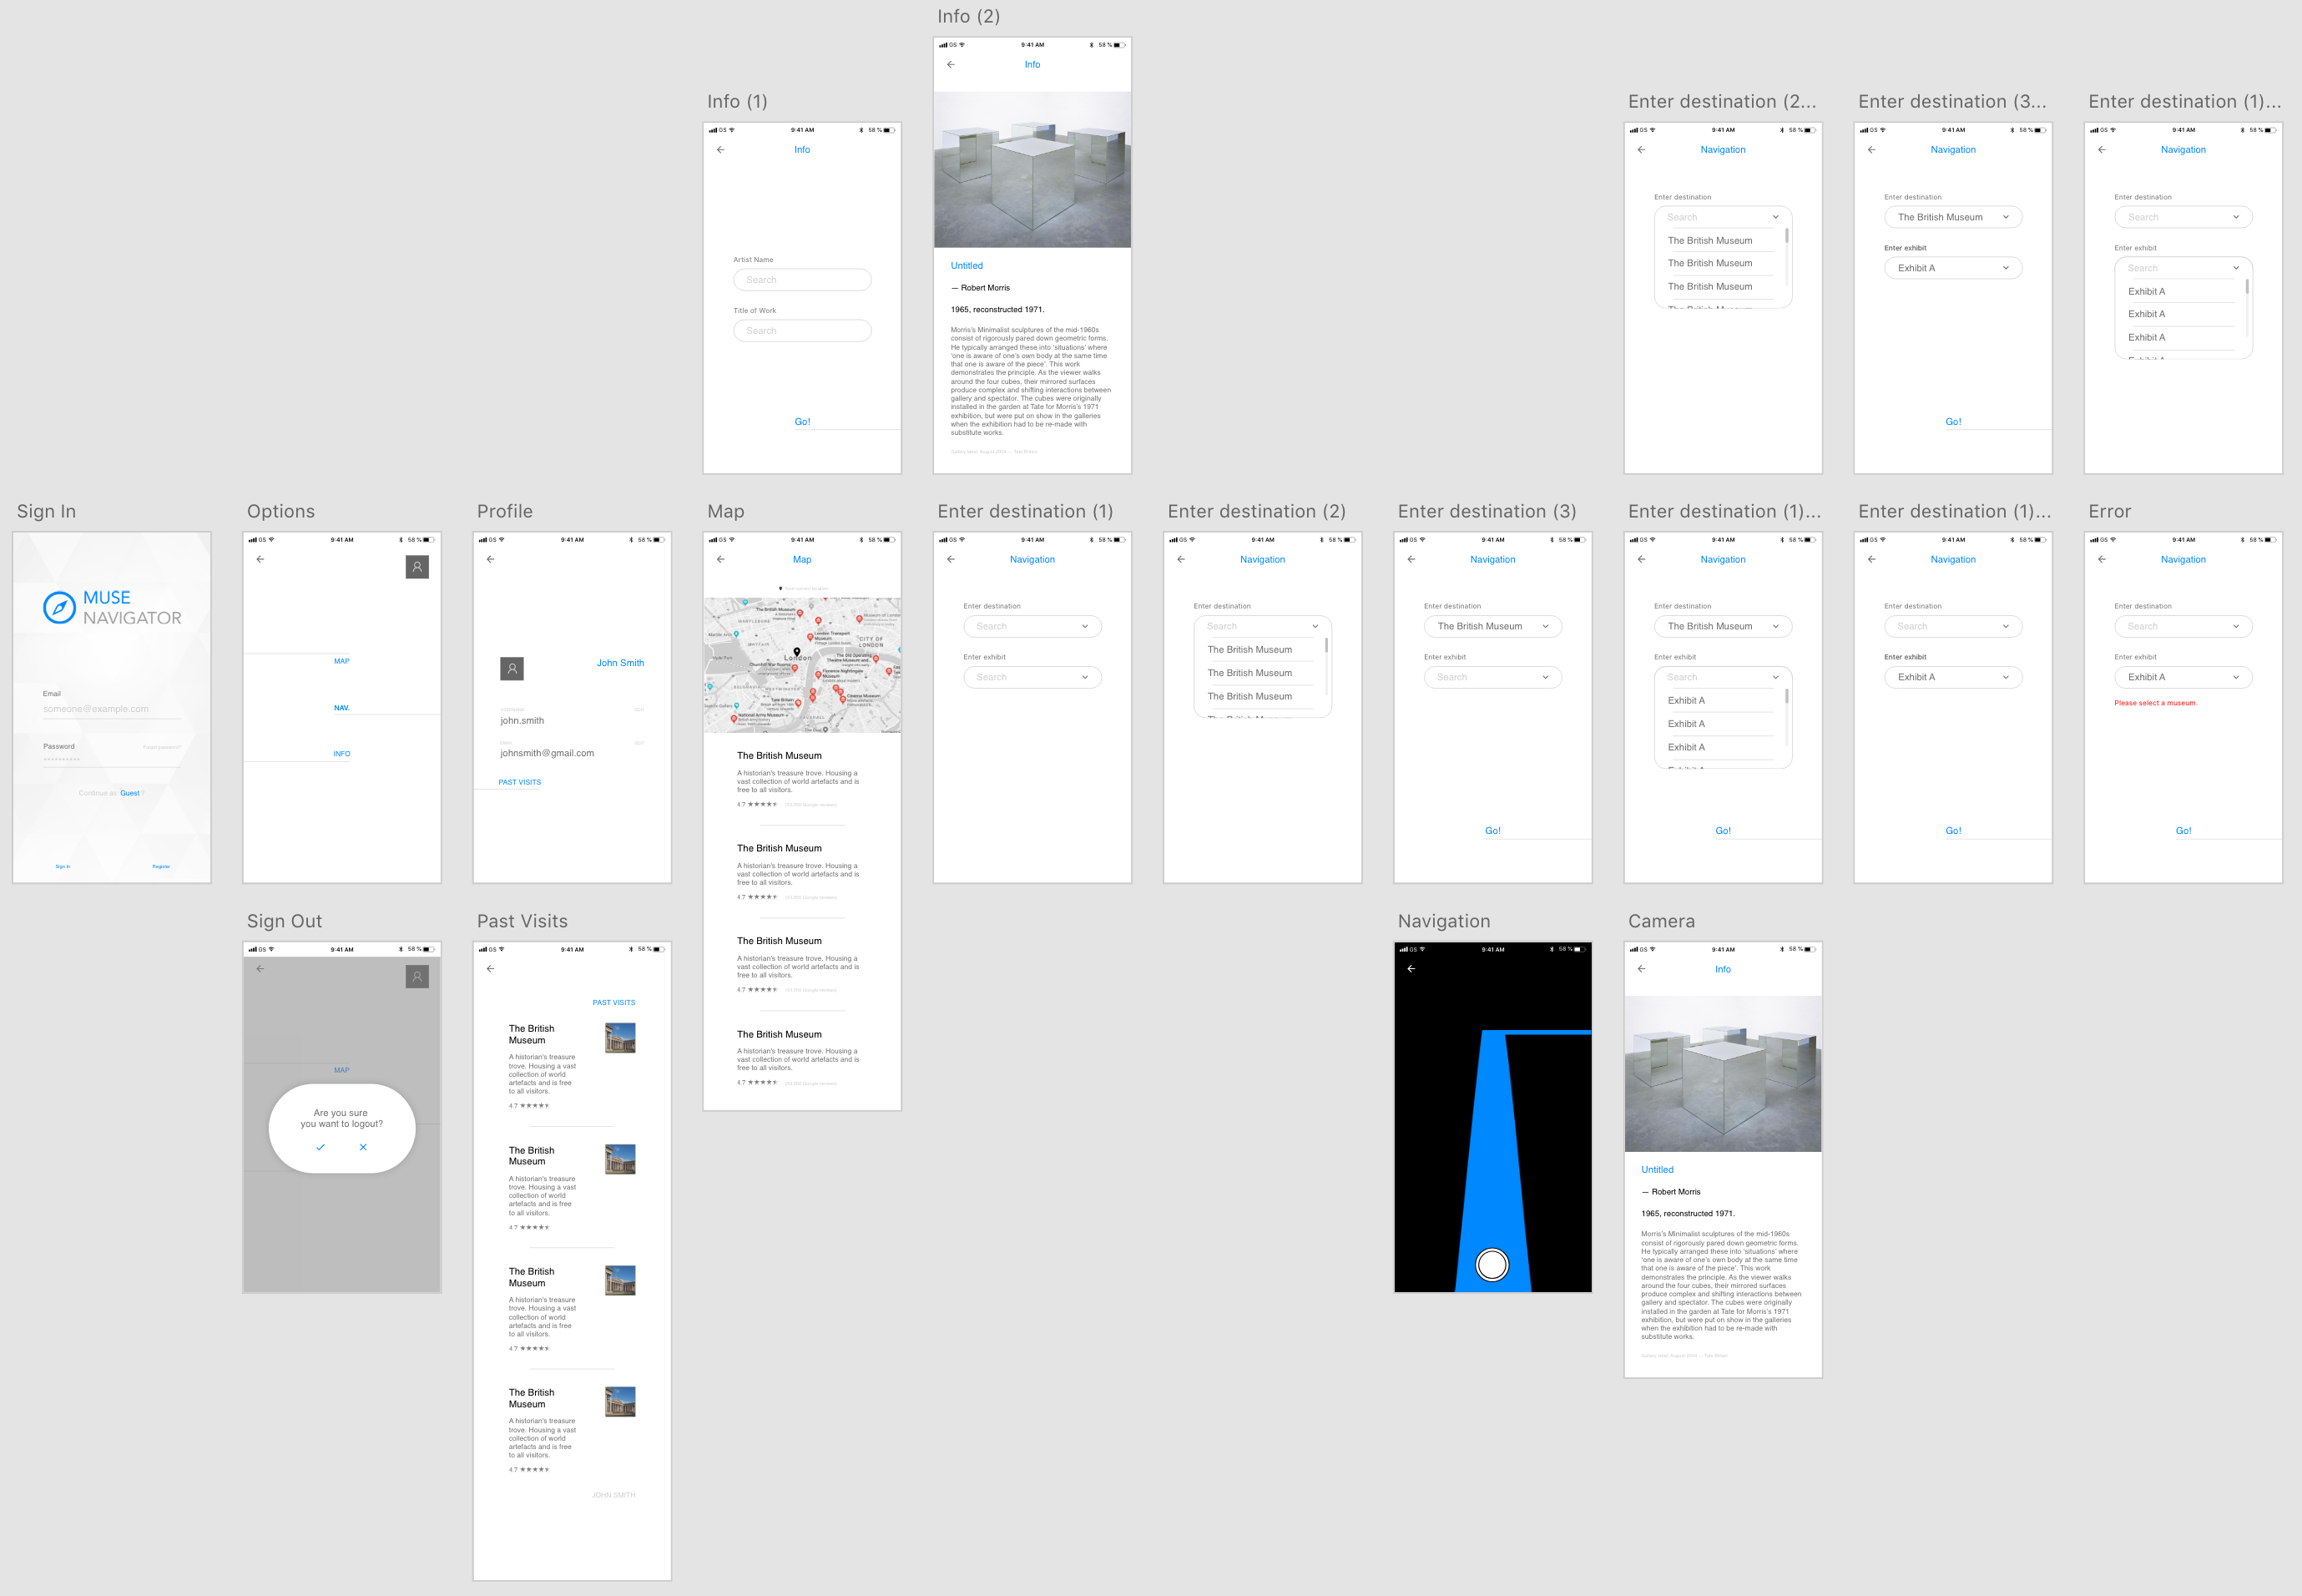
\includegraphics[angle=90, width=\textwidth]
    {prototypes/ui/final.png}
    \caption{Overview of final UI prototype}
    \label{fig:finaloverview}
\end{figure}

\newpage
\begin{figure}[H]
\centering
\begin{tabular}{cc}
  \includegraphics[width=60mm, height=100mm]{prototypes/ui/final/1.png} &   \includegraphics[width=60mm, height=100mm]{prototypes/ui/final/2.png} \\
(a) Sign in  & (b) Options \\[6pt]
 \includegraphics[width=60mm, height=100mm]{prototypes/ui/final/3.png} &   
\includegraphics[width=60mm, height=100mm]{prototypes/ui/final/4.png} \\
(c) Profile & (d) Past visits \\[6pt]
\end{tabular}
\caption{Final UI Designs of App}
\end{figure}

\newpage
\begin{figure}[H]
\centering
\begin{tabular}{cc}
  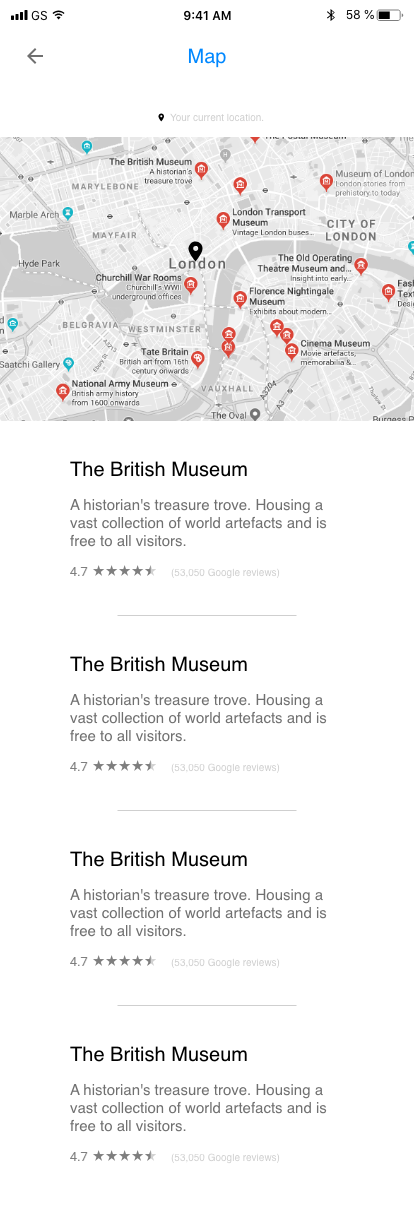
\includegraphics[width=60mm, height=100mm]{prototypes/ui/final/5.png} &   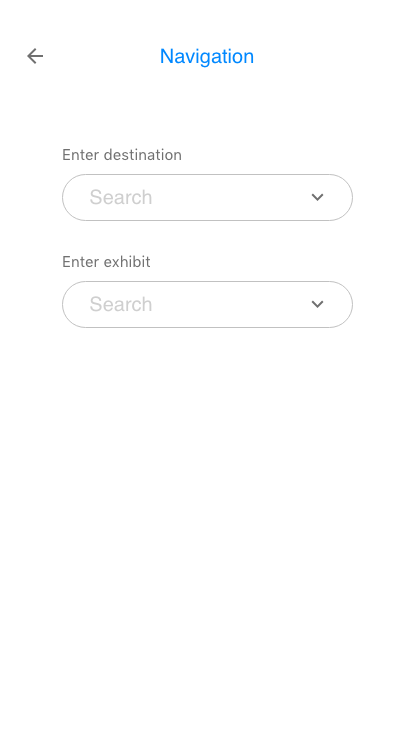
\includegraphics[width=60mm, height=100mm]{prototypes/ui/final/6a.png} \\
(e) Map of museums & (f) Destination \\[6pt]
 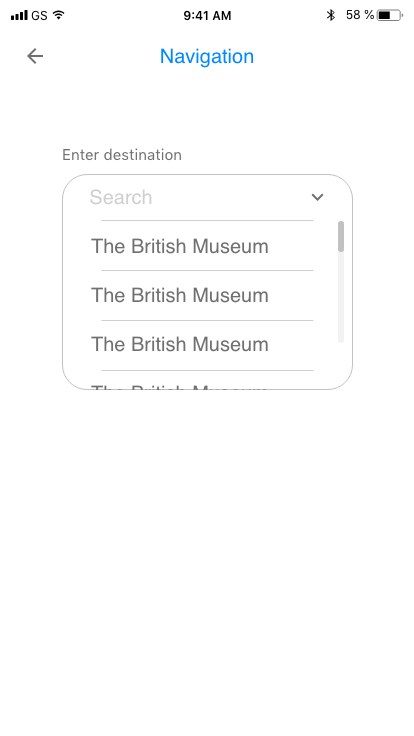
\includegraphics[width=60mm, height=100mm]{prototypes/ui/final/6b.png} &   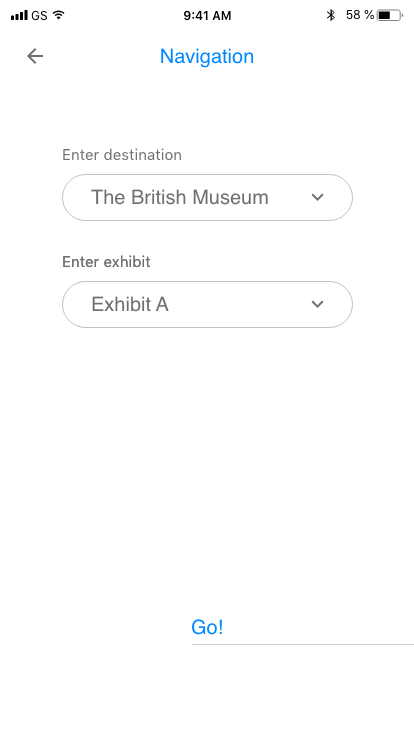
\includegraphics[width=60mm, height=100mm]{prototypes/ui/final/6c.png} \\
(g) Destination Dropdown & (h) Filled  \\[6pt]
\end{tabular}
\end{figure}

\newpage
\begin{figure}[H]
\centering
\begin{tabular}{cc}
  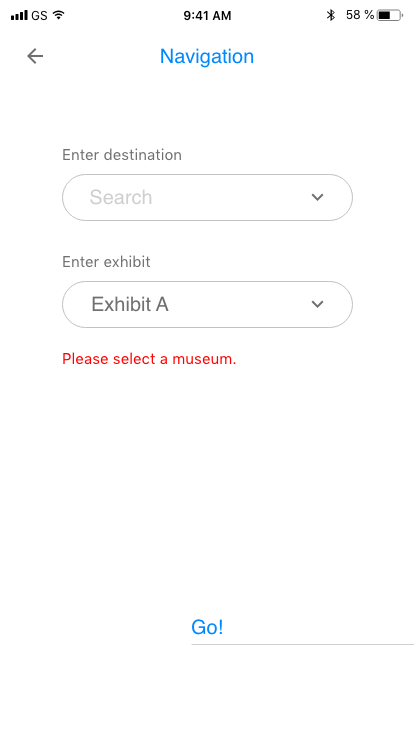
\includegraphics[width=60mm, height=100mm]{prototypes/ui/final/6d.png} &   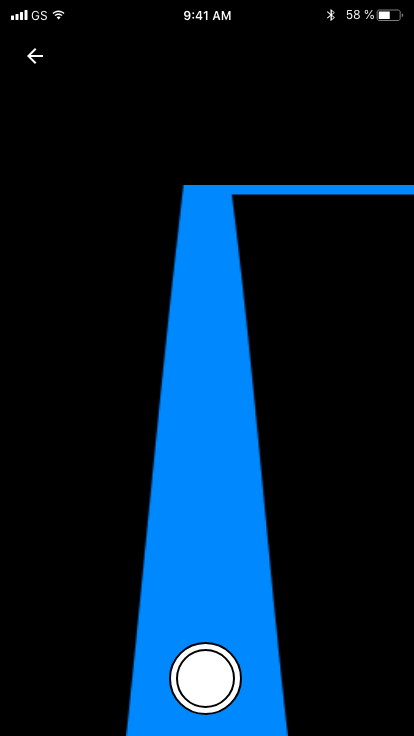
\includegraphics[width=60mm, height=100mm]{prototypes/ui/final/7.png} \\
(i) Error message & (j) AR Navigation \\[6pt]
 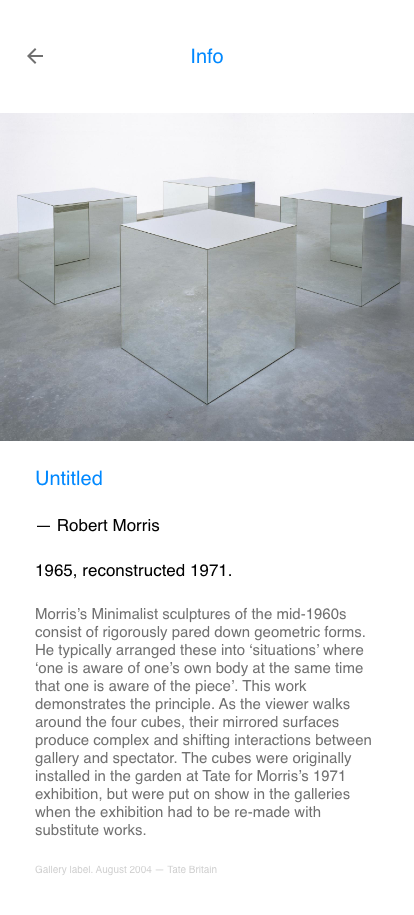
\includegraphics[width=60mm, height=100mm]{prototypes/ui/final/8.png} &   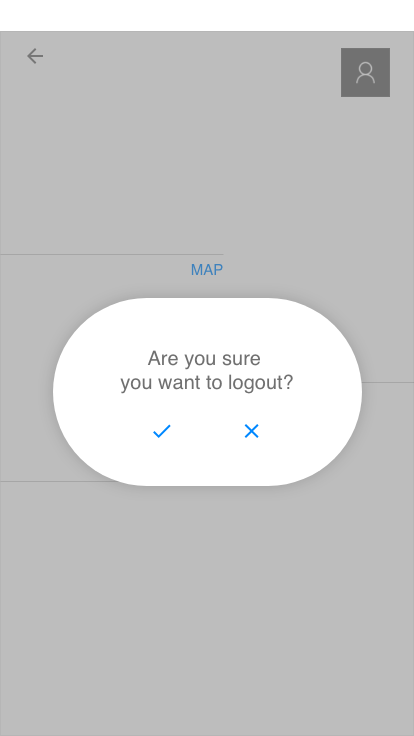
\includegraphics[width=60mm, height=100mm]{prototypes/ui/final/9.png} \\
(k) Artwork description & (l) Sign out \\[6pt]
\end{tabular}
\end{figure}

\newpage
\section{Technical Architecture}
\begin{figure}[H]
    \centering
    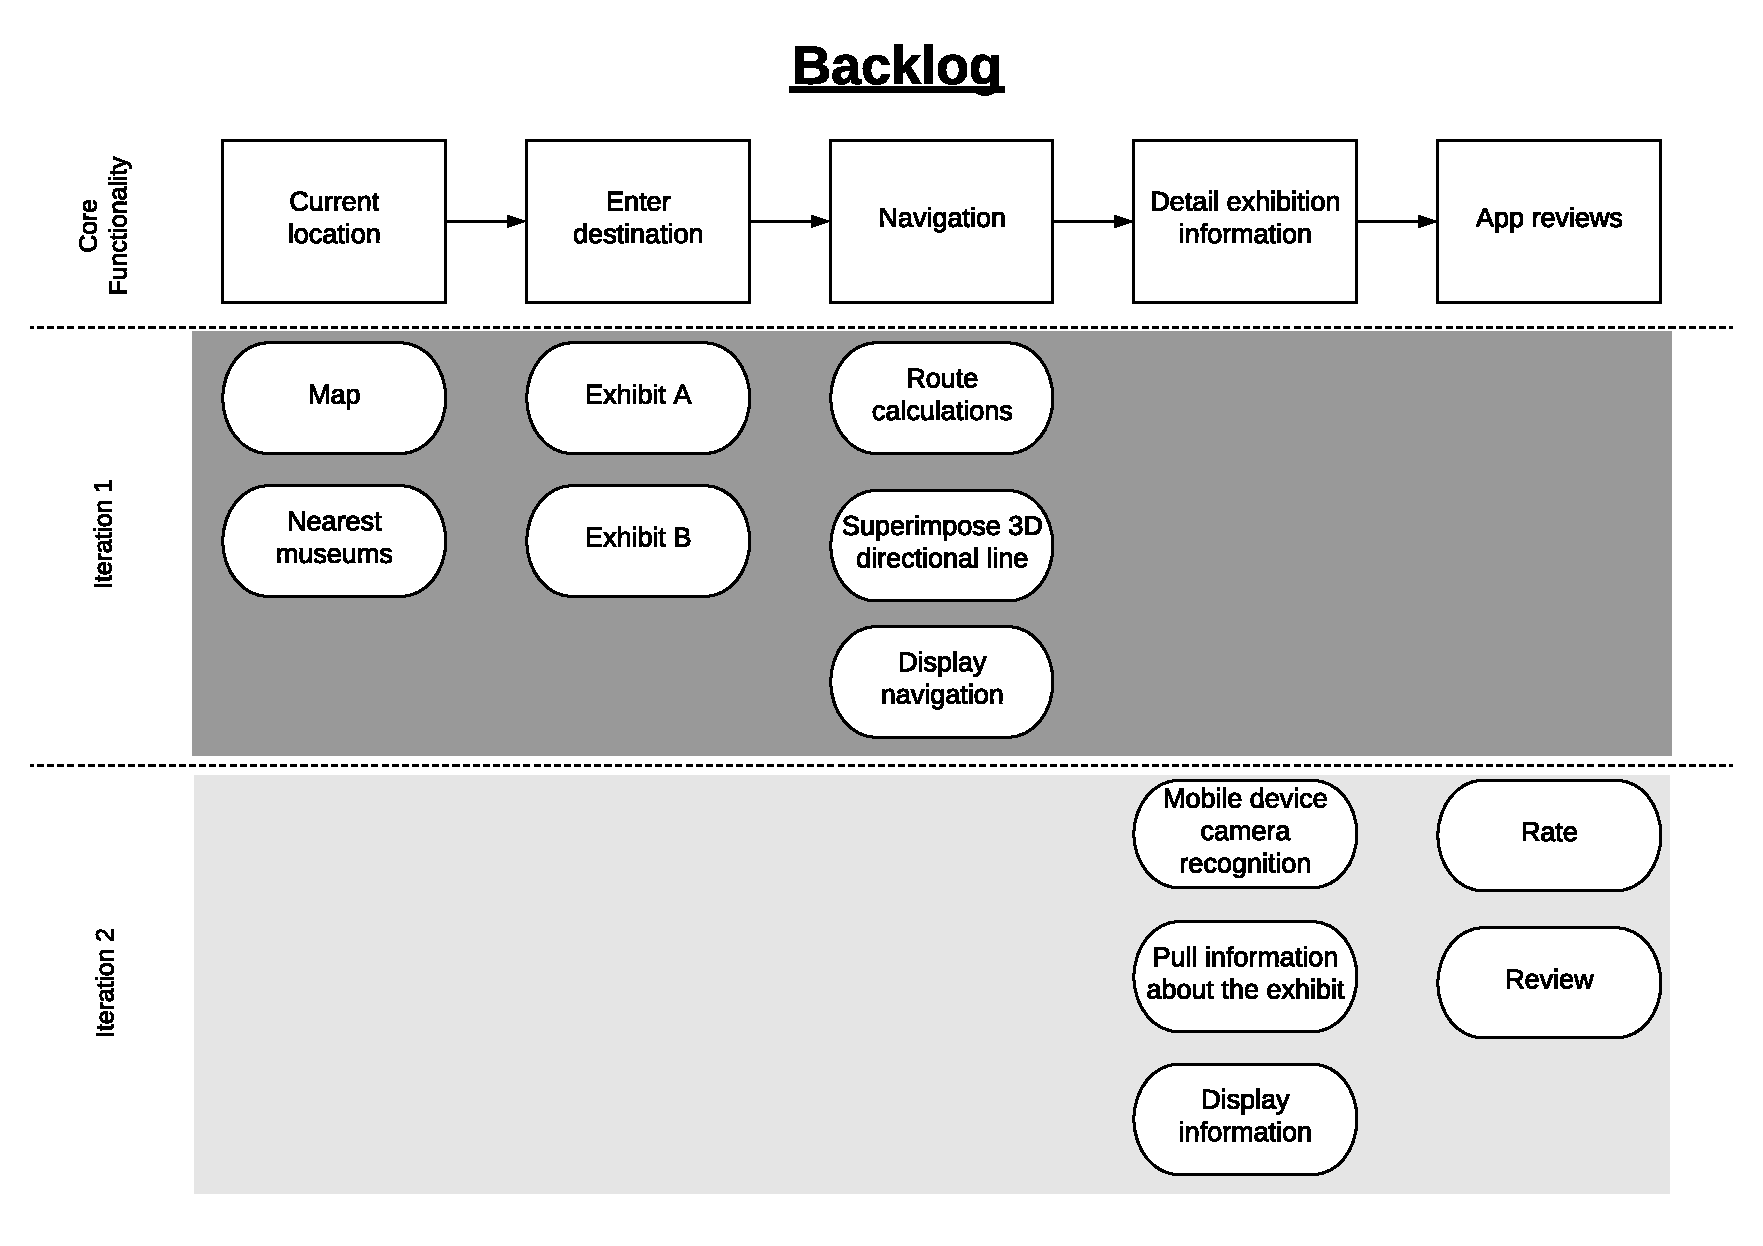
\includegraphics[width=\textwidth]
    {technicalarchitecture/backlog.pdf}
    \caption{Backlog Diagram}
    \label{fig:Backlog}
\end{figure}

\begin{figure}[H]
    \centering
    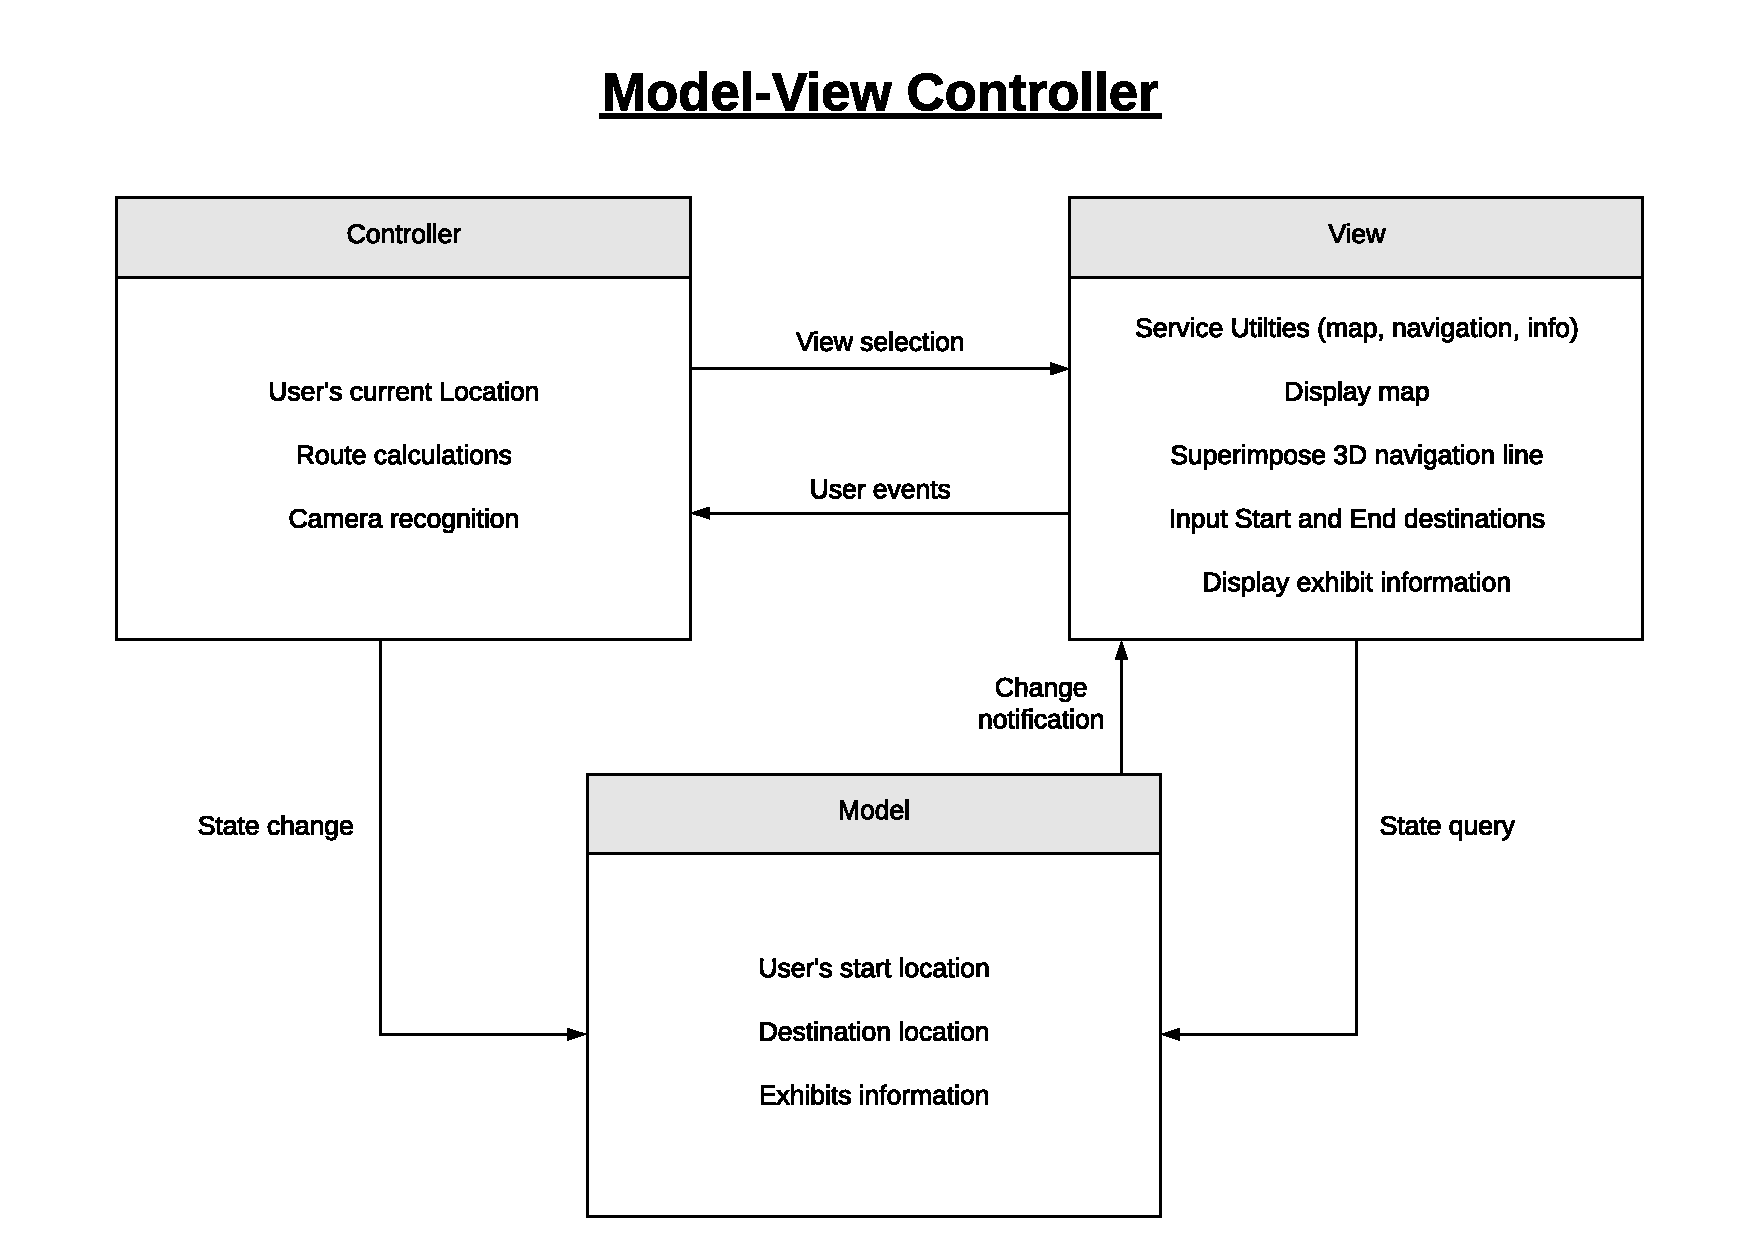
\includegraphics[width=\textwidth]
    {technicalarchitecture/mvc.pdf}
    \caption{Model-View Controller Diagram}
    \label{fig:MVC}
\end{figure}
